\documentclass{article}
\usepackage[utf8]{inputenc}
\usepackage{graphicx}
\title{SLDC Model}
\author{mehakp380 }
\date{September 2017}

\begin{document}

\begin{center}
    \large{\textbf{Software Development Lifecycle Models}}
\end{center}

Software development is a continuous process. It involves various phases which are to be completed for the complete development of the software. By using a software development lifecycle model in our project we make sure that our project works systematically and provides us the final product in a timely and cost effective manner.

The various phases which are included in the software development cycle are:
\begin{itemize}
    \item 	Feasibility
    \item 	Requirements Specification
    \item 	Design
    \item Coding and Unit Testing
    \item 	Integration 
    \item Testing
    \item Maintenance
\end{itemize}
Some of the lifecycle models we have assessed include:
\begin{itemize}
    \item 	Classical Waterfall model
    \item 	Iterative Waterfall model
    \item Prototyping model
    \item Coding and Unit Testing
    \item Rapid Application Development model
    \item 	Evolutionary model
    \begin{itemize}
    \item  Incremental model
    \item Spiral model
    \item Concurrent Development model 

\end{itemize}
\end{itemize}


Let us look at each of these models in detail and discuss the merits and demerits of each model.\\
\vspace{2cm}
\\\large{\textbf{Classical Waterfall model}}

This model is called the classical waterfall model because it diagrammatically represents a group of cascading waterfalls. It is a model in which each one of the lifecycle phases work in a sequential manner. This type of model requires user requirements to be understood very clearly and explicitly.\\

\textbf{Merits:}
\begin{itemize}
    \item Model is simple and easy to use.
    \item Model is effective when the problem is well understood.
    \item Rigidity of the model makes adhering to deadlines easier.
    \item 	Model works better for smaller projects.

\end{itemize}
\textbf{De-Merits:}

\begin{itemize}
    \item 		In this model reverting back to previous phases is costly and not feasible.
    \item 	Huge amount of risk.
    \item 	It requires all requirements to be stated explicitly.
    \item  Difficult to accommodate uncertainty.
    \item 	A major mistake is as good as an irreversible mistake.

 \end{itemize}
 \vspace{1cm}
\begin{figure}
  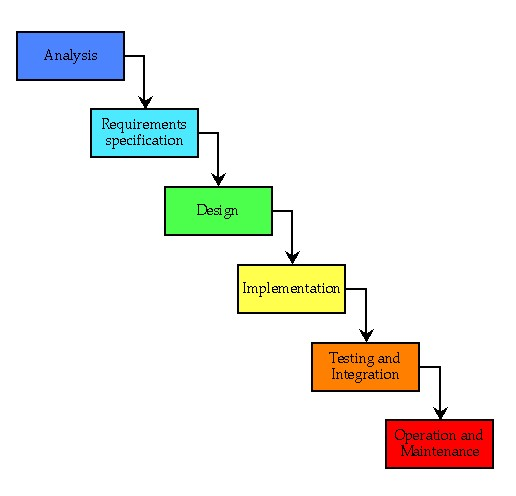
\includegraphics[width=10cm, height=8cm]{fig1.jpg}
  \caption{Classical waterfall model - Diagrammatic representation}
  
\end{figure}
\vspace{7cm}

\large{\textbf{Iterative Waterfall Model}}

An iterative waterfall model works on the principle that the errors should be detected and rectified as soon as possible. In this model one can go the previous phase where the error can be detected to ensure that all the previous phases uptil now are error free. \\

\textbf{Merits:}
\begin{itemize}
    \item 			If the errors are detected at an early stage, this model becomes extremely systematic and easy to implement.
    \item Results are obtained periodically.
    \item Risk are identified and resolved during iteration.
    \item  	Easy to measure progress.
    \item 	Supports changing requirements.
    \item 	Easy to measure progress.

    \end{itemize}
\vspace{1.5cm}
\textbf{Demerits:}
\begin{itemize}
   \item 	If errors are not detected early, the whole development model fails.
 \item 	More management is needed.

\end{itemize}
 \begin{figure}
  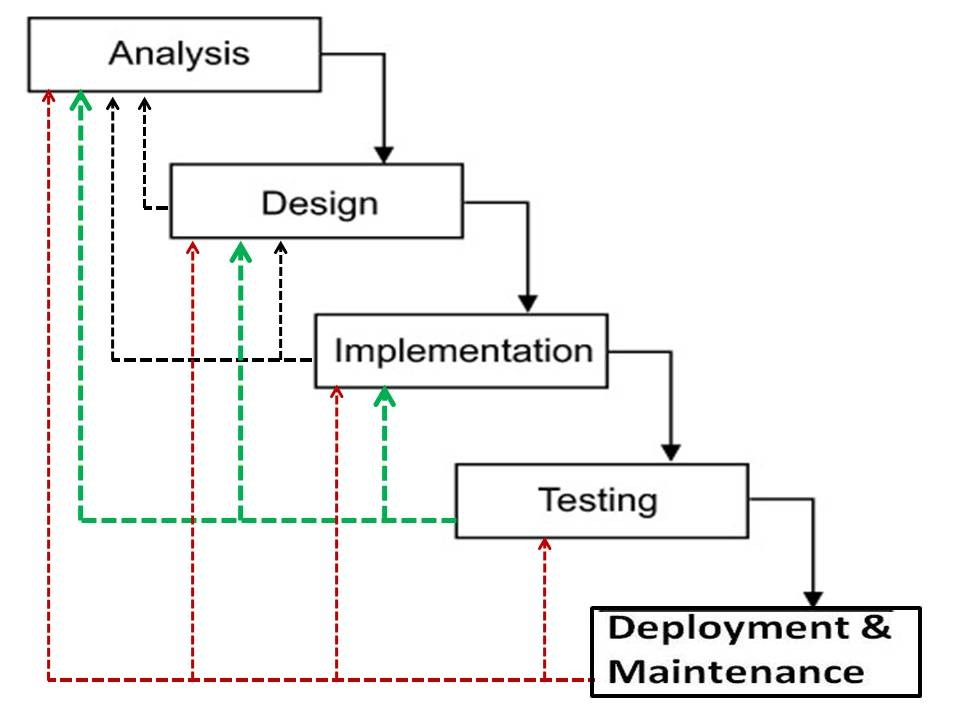
\includegraphics[width=10cm, height=7cm]{fig2.jpg}
  \caption{Iterative Waterfall Diagram}
  
\end{figure}
\vspace{0.5cm}

\large{\textbf{Software Prototype Model}}

A system prototype refers to a working model of the system. A prototype gives an idea about the functionality of the system but it does not contain the exact logic of the system. Software prototyping is done to provide the user with an idea of what the system is and how it will work. It is done to ensure that the user is satisfied with the system’s functionality before the actual implementation of the system.\\

Below is a diagram representing the different phases of this model.\\
\begin{figure}
  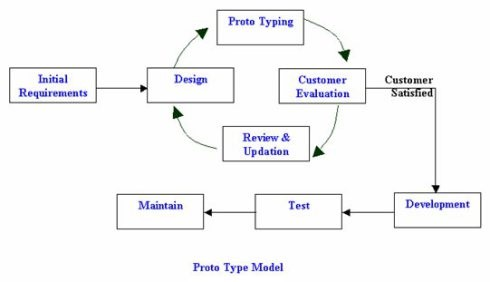
\includegraphics[width=10cm, height=7cm]{fig3.jpg}
  \caption{Software Prototype Model}
  
\end{figure}
 


\vspace{5cm}
Let us look at the merits and demerits of using such a model.\\

\textbf{Merits:}
\begin{itemize}
    


\item 	This models ensures better involvement of users in the development process which is always a good thing.
\item 	This model reduces cost and time as defects in the features and functionality can be detected and rectified at an early stage.
\item 	Since a working model of the system is provided to the user, he/she gets a better idea of the system being built and he can state his requirements more clearly.
\item Missing functionality or misinterpreted functionality can be detected easily.
\end{itemize}

\textbf{Demerits:}
\begin{itemize}
    
\item If the prototype development process is not coordinated, this can consume a lot more time than any other model.
\item 	As there is too much dependency on the prototype, there is a risk of requirements analysis becoming inefficient.
\item 	If there are a large number of prototypes, the user may get confused.
\item 	Developing a prototype is dependent on the skills and understanding of the development team. Hence this model becomes inefficient for totally new development environments and new areas of development.
\item 	Developers may use the existing prototypes to make the actual system even when it is not technically feasible. 
 
\end{itemize}
\vspace{0.5cm}
\large{\textbf{Spiral Model }}

The spiral model combines the idea of iterative development with the systematic, controlled aspects of the waterfall model. Spiral model is a combination of iterative development process model and sequential linear development model i.e. waterfall model with very high emphasis on risk analysis. It allows for incremental releases of the product, or incremental refinement through each iteration around the spiral.\\

Each loop has four sections or quadrants :\\
\begin{enumerate}
    

\item To determine the objectives, alternatives and constraints: We try to understand the product objectives, alternatives in design and constraints imposed because of cost, technology, schedule, etc.

\item  Risk analysis and evaluation of alternatives: Here we try to find which other approaches can be implemented in order to fulfill the identified constraints. Operational and technical issues are addressed here. Risk mitigation is in focus in this phase. And evaluation of all these factors determines future action.

\item  Execution of that phase of development: In this phase we develop the planned product. Testing is also done. In order to do development, waterfall or incremental approach can be implemented.

\item  Planning the next phase: Here we review the progress and judge it considering all parameters. Issues which need to be resolved are identified in this phase and necessary steps are taken.
\end{enumerate}
 \begin{figure}
  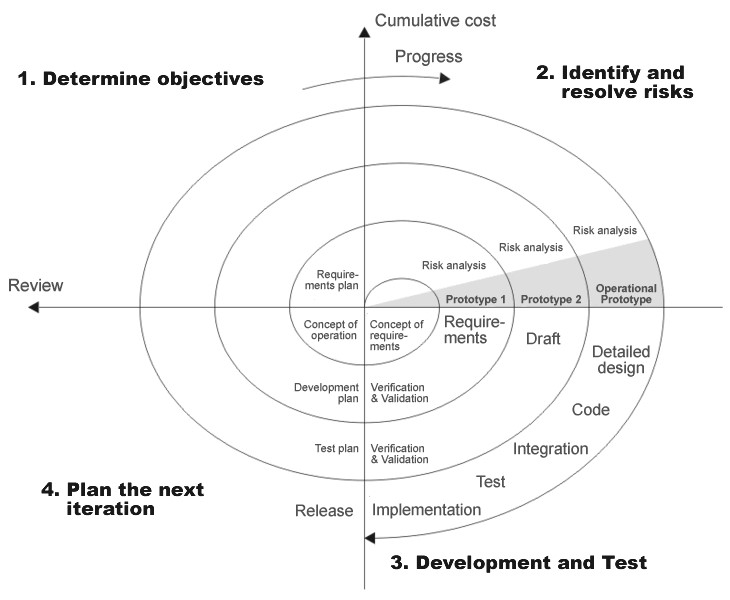
\includegraphics[width=10cm, height=8cm]{fig4.jpg}
  \caption{Spiral Model }
  
\end{figure}
 
\textbf{NOTE :}
\textit{
Radius of the spiral (at any point) indicates the cost incurred on the project (so far). Angular dimension represents progress.}


\textbf{Merits:}
\begin{itemize}
   \item 	Changing requirements can be accommodated later.
 \item 	Software is produced early in the software life cycle.
 \item 	Development can be divided into smaller parts and more risky parts can be developed earlier which helps better risk management.
\end{itemize}
\textbf{De-Merits:}
\begin{itemize}
 \item 	Project’s success is highly dependent on the risk analysis phase.
 \item 	Process is complex as large number of intermediate stages requires excessive documentation.
 \item 	Spiral may go indefinitely.
 \item 	Not suitable for small or low risk projects and could be expensive for small projects.
\end{itemize}

\textbf{ When to use Spiral model:}
 \begin{itemize}
 \item 	When costs and risk evaluation is important
 \item 	For medium to high-risk projects
 \item 	Long-term project commitment unwise because of potential changes to economic priorities
 \item 	Users are unsure of their needs
 \item 	Requirements are complex
 \item 	Significant changes are expected (research and exploration)


\end{itemize}
\vspace{0.5cm}

\large{\textbf{Concurrent Development Model}}
\vspace{0.2cm}
It is suitable for all types of software but is generally used for client server applications. It provides a precise state of the current state of the project. Rather than confining software engineering activities to a sequence of events, it defines a network of activities. Each activity on the network exists simultaneously with other activities. It focuses on concurrent development activities such as prototyping, analysis modeling, requirements specifications and design. The model can be represented systematically as a series of major technical activities, tasks and their associated states. Events generated at one point in the process network trigger transitions among the states.

\begin{figure}
  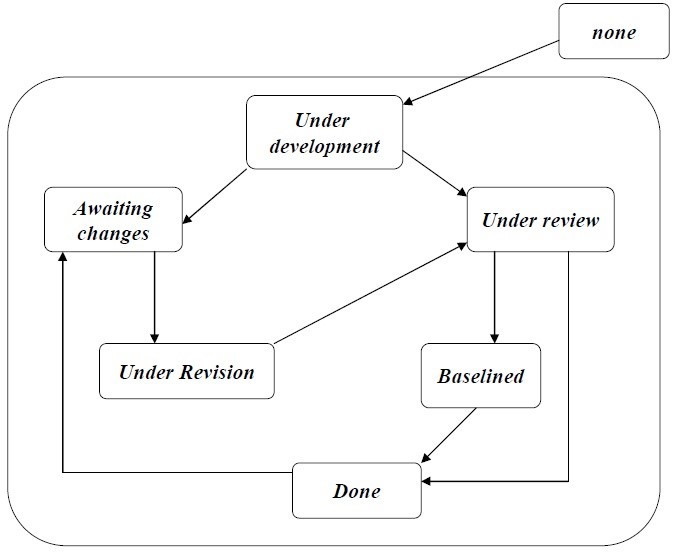
\includegraphics[width=10cm, height=6cm]{fig5.jpg}
  \caption{Concurrent Development Model }
  
\end{figure}
\textbf{Merits:}
\begin{itemize}
    

\item 	Applicable to all types of softwares.
\item 	Gives precise state of the project at a given time.
\item 	Defines a series of events that will trigger transition from state to state for each of the software engineering activities and action or task.
\end{itemize}
\textbf{De-Merits:}
\begin{itemize}
\item 	The SRS document must be continuously updated to reflect the changes.
\item 	It is inconvenient to avoid adding too many new features at later stages of software development.
\end{itemize}
\vspace{0.5cm}
\large{\textbf{Incremental Model}}

Incremental build model is a method of software development where product is designed, implemented and tested incrementally until the product is finished.The product is defined  as finished when it satisfies all the requirements. In this model the product is decomposed into number of component, each of which is designed and build separately. Each component is delivered to client when it is complete. The incremental model applies the waterfall model incremental. \\
 
\begin{figure}
  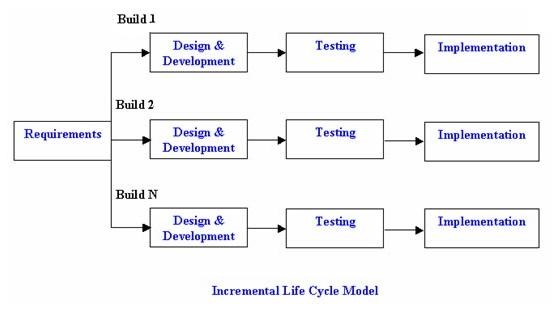
\includegraphics[width=10cm, height=7cm]{fig6.jpg}
  \caption{Incremental Model }
  
\end{figure}
Let us look at the merits and demerits of using such a model.\\
\textbf{Merits:}
\begin{itemize}
\item 	Generates working  software quickly and early during the software life cycle.
\item 	This model is more flexible – less costly to change scope and requirements.
\item	It is easier to test and debug during a smaller iteration.
\item	Customer can respond to features and review the product for any needful changes.
\end{itemize}
\vspace{4cm}
\textbf{De-Merits:}
\begin{itemize}
\item	Resulting Cost may exceed the cost of the organization.
\item	This model require good planning and design.
\item	In this, we require complete and clear definition of whole system before, It can be broken down and build incrementally.
\end{itemize}

\vspace{0.5cm}
\large{\textbf{Evolutionary Software Development Model}}

The ESD model divides the developmental cycle into smaller incremental waterfall models in which users are able to get access to the product at the end of each cycle. The users provide feedback on the product for the planning stage of the next cycle and the development team responds, often by changing the product,plans or processes.
 \begin{figure}
  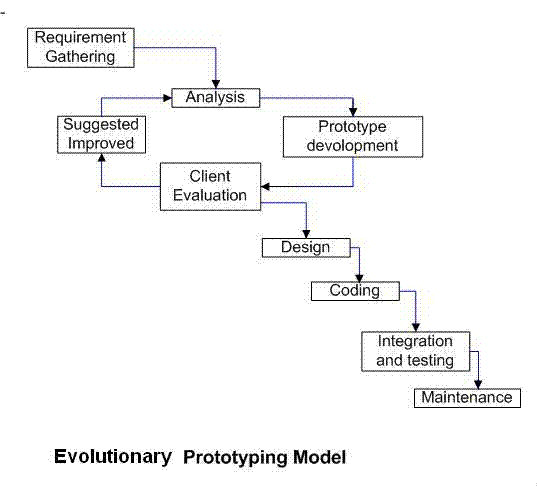
\includegraphics[width=10cm, height=7cm]{fig7.png}
  \caption{Evolutionary Software Development Model}
  
\end{figure}
\vspace{6cm}
\\\textbf{Merits:}
\begin{itemize}
\item	There is a significant reduction in risk for software projects as by breaking the project into smaller pieces and increasing the visibility of management would ensure that these risks can be addressed and managed. 
\item	ESD can reduce costs by providing a structured and a disciplined way for testing project
\item	It supports changing requirements and the Initial Operating time is less.
\item	Shorter cycles result in a more thorough and frequent improvement process. 
\end{itemize}
\textbf{De-Merits:}
\begin{itemize}
\item	Not suitable for smaller projects.
\item	Management complexity is more.
\item	End of project may not be determined which is a risk.
\item	Highly skilled resources are required for risk analysis.
\item	Project's progress is highly dependent upon the risk analysis phase.
\end{itemize}


\vspace{0.5cm}

\large{\textbf{Rapid Application development (RAD)}}

Rapid application development RAD is a software development methodology that uses minimal planning in favor of rapid prototyping. A prototype is a working model that is functionally equivalent to a component of the product.
In RAD model the functional modules are developed in parallel as prototypes and are integrated to make the complete product for faster product delivery.

Since there is no detailed preplanning, it makes it easier to incorporate the changes within the development process. RAD projects follow iterative and incremental model and have small teams comprising of developers, domain experts, customer representatives and other IT resources working progressively on their component or prototype.\\
\begin{figure}
  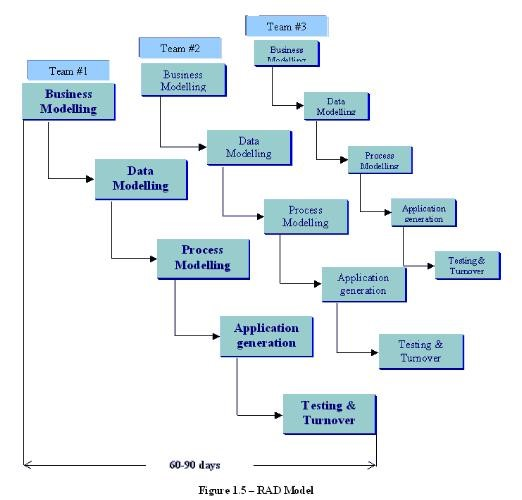
\includegraphics[width=10cm, height=7cm]{fig8.jpg}
  \caption{Rapid Application development }
  
\end{figure}
\vspace{13cm}
\\\textbf{Merits:}
\begin{itemize}
\item	Changing requirements can be accommodated.
\item	Progress can be measured.
\item	Iteration time can be short with use of powerful RAD tools.
\item	Productivity with fewer people in short time.
\item	Reduced development time.
\item	Increases reusability of components
\item	Quick initial reviews occur
\item	Encourages customer feedback
\item	Integration from very beginning solves a lot of integration issues.
\end{itemize}
\textbf{De-Merits:} 
\begin{itemize}
\item	Dependency on technically strong team members for identifying project requirements.
\item	Only system that can be modularized can be built using RAD.
\item	Requires highly skilled developers/designers.
\item	High dependency on modeling skills.
\item	Inapplicable to cheaper projects as cost of modeling and automated code generation is very high.
\item	Management complexity is more.
\item	Suitable for systems that are component based and scalable.
\item	Requires user involvement throughout the life cycle.
\item	Suitable for project requiring shorter development times

 \end{itemize}

\large{\textbf{Conclusion:}}

Decided Model 



\end{document}
